%===========================================================================


\section{Clinical Utility: Net Benefit, Operating Points, and Event-Level
    Detection}
\label{sec:clinical_utility}
%===========================================================================

This section reports four operational quantities: net benefit across a
plausible threshold range, the positive predictive value and false-alarm
rate at a fixed sensitivity, detection expressed per patient rather than per
person-hour, and the lead time gained when detection occurs.

Under the discrete-time competing-risks specification, $\text{event}=1$ marks
the onset hour itself, so each septic stay contributes one event hour out of a
mean of 45. Per-hour sensitivity requires the alert to fire \emph{in the onset
hour}; per-patient sensitivity asks only whether the patient was alerted before
onset. Per-hour figures alone understate detection and do not show the
associated alarm volume.

\subsection{Decision-Curve Analysis \texorpdfstring{[C]}{[C]}}

Decision-curve analysis requires a threshold grid, and at this prevalence the
choice of grid determines the result. A threshold probability of $t$ encodes a willingness to accept
$(1-t)/t$ false alarms per true detection. The hourly event rate here is
0.19--0.42 per cent, so the conventional grid of 0.01--0.20 sits between five
and one hundred times the prevalence: at $t=0.01$ the analyst is asserting a
tolerance of only 99 false alarms per detection, far below what an hourly
sepsis alert must absorb, and every curve falls trivially below ``treat
none''. Net benefit is therefore evaluated on a grid from one tenth to ten
times the prevalence, following Vickers and Elkin \cite{vickers2006dca}.

\begin{figure}[H]
    \centering
    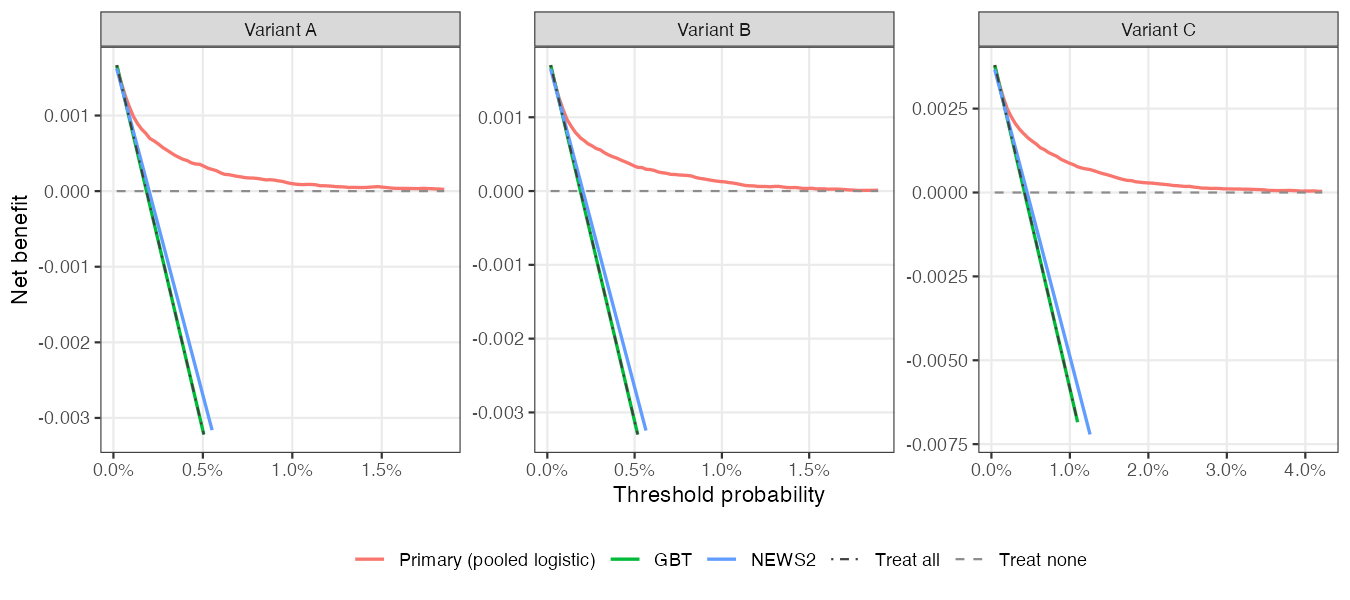
\includegraphics[width=\textwidth]{images/11_decision_curves.png}
    \caption{Decision curves on the temporal test set. Net benefit against
    threshold probability, with both default strategies shown. Curves are
    clipped below $-1.75\times$ prevalence for legibility.}
    \label{fig:decision_curves}
\end{figure}

\begin{table}[H]
    \centering\small
    \begin{tabular}{llrrrr}
        \toprule
        \textbf{Var} & \textbf{Model} & \textbf{Net benefit}
        & \textbf{Std NB} & \textbf{Alert rate} & \textbf{Alert-rate span} \\
        \midrule
        A & Primary & \pcNetBenefitPrimaryA & \pcSnbPrimaryA & \pcAlertRatePrimaryA & \pcAlertRangePrimaryA \\
        A & GBT     & \pcNetBenefitGbtA & \pcSnbGbtA & \pcAlertRateGbtA & \pcAlertRangeGbtA \\
        A & Cox     & \pcNetBenefitCoxA & \pcSnbCoxA & \pcAlertRateCoxA & \pcAlertRangeCoxA \\
        A & NEWS2   & \pcNetBenefitNewsA & \pcSnbNewsA & \pcAlertRateNewsA & \pcAlertRangeNewsA \\
        A & qSOFA   & \pcNetBenefitQsofaA & \pcSnbQsofaA & \pcAlertRateQsofaA & \pcAlertRangeQsofaA \\
        A & SIRS    & \pcNetBenefitSirsA & \pcSnbSirsA & \pcAlertRateSirsA & \pcAlertRangeSirsA \\
        \midrule
        B & Primary & \pcNetBenefitPrimaryB & \pcSnbPrimaryB & \pcAlertRatePrimaryB & \pcAlertRangePrimaryB \\
        B & GBT     & \pcNetBenefitGbtB & \pcSnbGbtB & \pcAlertRateGbtB & \pcAlertRangeGbtB \\
        B & Cox     & \pcNetBenefitCoxB & \pcSnbCoxB & \pcAlertRateCoxB & \pcAlertRangeCoxB \\
        B & NEWS2   & \pcNetBenefitNewsB & \pcSnbNewsB & \pcAlertRateNewsB & \pcAlertRangeNewsB \\
        B & qSOFA   & \pcNetBenefitQsofaB & \pcSnbQsofaB & \pcAlertRateQsofaB & \pcAlertRangeQsofaB \\
        B & SIRS    & \pcNetBenefitSirsB & \pcSnbSirsB & \pcAlertRateSirsB & \pcAlertRangeSirsB \\
        \midrule
        C & Primary & \pcNetBenefitPrimaryC & \pcSnbPrimaryC & \pcAlertRatePrimaryC & \pcAlertRangePrimaryC \\
        C & GBT     & \pcNetBenefitGbtC & \pcSnbGbtC & \pcAlertRateGbtC & \pcAlertRangeGbtC \\
        C & Cox     & \pcNetBenefitCoxC & \pcSnbCoxC & \pcAlertRateCoxC & \pcAlertRangeCoxC \\
        C & NEWS2   & \pcNetBenefitNewsC & \pcSnbNewsC & \pcAlertRateNewsC & \pcAlertRangeNewsC \\
        C & qSOFA   & \pcNetBenefitQsofaC & \pcSnbQsofaC & \pcAlertRateQsofaC & \pcAlertRangeQsofaC \\
        C & SIRS    & \pcNetBenefitSirsC & \pcSnbSirsC & \pcAlertRateSirsC & \pcAlertRangeSirsC \\
        \bottomrule
    \end{tabular}
    \caption{Net benefit at a threshold probability equal to the event
    prevalence. At that threshold both defaults have net benefit exactly zero
    and the maximum attainable net benefit is the prevalence itself, so
    standardised net benefit (Std NB = net benefit / prevalence) is the
    fraction of the attainable benefit captured. ``Alert-rate span'' is the
    change in alert rate across the threshold grid.}
    \label{tab:net_benefit}
\end{table}

Decision-curve analysis produced positive but modest net benefit for the
primary model. At a threshold equal to the prevalence, the primary model captures
\pcSnbPctPrimaryA\% (Variant A), \pcSnbPctPrimaryB\% (Variant B) and
\pcSnbPctPrimaryC\% (Variant C) of the attainable net benefit. The three
variants span barely three percentage points, so, unlike discrimination, this
share is insensitive to the reading of Sepsis-3. The qualitative result matches
the swept Utility Score (Table~\ref{tab:utility_optimum}): a small positive
margin for the fitted models and none for the rule-based comparators. The
magnitudes differ because the metrics price errors differently: net benefit
weights a false alarm by $t/(1-t)$, which at $t = \pcPrevalenceB$ is very
small, whereas the Utility Score imposes a fixed $-0.05$ penalty per
false-alert hour. Net benefit is therefore the more generous metric here, and
the gap widens as the alert rate rises. The preferred weighting of false alerts
depends on the intended clinical decision and should be specified before
deployment. This within-cohort disagreement is not an instance of H5's
internal-to-external estimand.

For every model except the primary one, the alert-rate span is zero across the
plausible threshold range. GBT and Cox alert on \emph{100\% of person-hours} at
every threshold in this range, so their decision curves coincide with treating
everyone (Figure~\ref{fig:decision_curves}); with predicted probabilities in
the 0.2--0.9 range (Table~\ref{tab:calibration}), no threshold below 4 per cent
excludes anything. NEWS2, qSOFA and SIRS are non-tunable for the opposite
reason: their integer scores map to a few fixed probabilities, all above the
grid, and they alert on a constant 58--86 per cent of person-hours. Within the
clinically plausible range, the primary model is therefore the only one whose
alert rate responds to the threshold; GBT's best operating point lies far above
that range (Table~\ref{tab:utility_optimum}).

\subsection{Operating Points at Fixed Sensitivity \texorpdfstring{[E]}{[E]}}
\label{sec:operating_points}

Alerting systems are usually commissioned by choosing a sensitivity target
rather than a fixed cut-off. Table~\ref{tab:operating_points} sets the threshold to the
largest cut-off achieving 80 per cent per-hour sensitivity and reads off the
resulting operating characteristics.

\begin{table}[H]
    \centering\small
    \adjustbox{max width=\textwidth}{%
    \begin{tabular}{llrrrrrr}
        \toprule
        \textbf{Var} & \textbf{Model} & \textbf{Specificity} & \textbf{PPV}
        & \textbf{NNE} & \textbf{Alerts/pt-day} & \textbf{FA/pt-day}
        & \textbf{FP:TP} \\
        \midrule
        A & Primary & \pcSpecPrimaryA & \pcPpvPrimaryA & \pcNnePrimaryA & \pcAlertsPerPtDayPrimaryA & \pcFaPerPtDayPrimaryA & \pcFpTpRatioPrimaryA \\
        A & GBT     & \pcSpecGbtA & \pcPpvGbtA & \pcNneGbtA & \pcAlertsPerPtDayGbtA & \pcFaPerPtDayGbtA & \pcFpTpRatioGbtA \\
        A & NEWS2   & \pcSpecNewsA & \pcPpvNewsA & \pcNneNewsA & \pcAlertsPerPtDayNewsA & \pcFaPerPtDayNewsA & \pcFpTpRatioNewsA \\
        A & Cox     & \pcSpecCoxA & \pcPpvCoxA & \pcNneCoxA & \pcAlertsPerPtDayCoxA & \pcFaPerPtDayCoxA & \pcFpTpRatioCoxA \\
        \midrule
        B & Primary & \pcSpecPrimaryB & \pcPpvPrimaryB & \pcNnePrimaryB & \pcAlertsPerPtDayPrimaryB & \pcFaPerPtDayPrimaryB & \pcFpTpRatioPrimaryB \\
        B & GBT     & \pcSpecGbtB & \pcPpvGbtB & \pcNneGbtB & \pcAlertsPerPtDayGbtB & \pcFaPerPtDayGbtB & \pcFpTpRatioGbtB \\
        B & NEWS2   & \pcSpecNewsB & \pcPpvNewsB & \pcNneNewsB & \pcAlertsPerPtDayNewsB & \pcFaPerPtDayNewsB & \pcFpTpRatioNewsB \\
        B & Cox     & \pcSpecCoxB & \pcPpvCoxB & \pcNneCoxB & \pcAlertsPerPtDayCoxB & \pcFaPerPtDayCoxB & \pcFpTpRatioCoxB \\
        \midrule
        C & Primary & \pcSpecPrimaryC & \pcPpvPrimaryC & \pcNnePrimaryC & \pcAlertsPerPtDayPrimaryC & \pcFaPerPtDayPrimaryC & \pcFpTpRatioPrimaryC \\
        C & GBT     & \pcSpecGbtC & \pcPpvGbtC & \pcNneGbtC & \pcAlertsPerPtDayGbtC & \pcFaPerPtDayGbtC & \pcFpTpRatioGbtC \\
        C & NEWS2   & \pcSpecNewsC & \pcPpvNewsC & \pcNneNewsC & \pcAlertsPerPtDayNewsC & \pcFaPerPtDayNewsC & \pcFpTpRatioNewsC \\
        C & Cox     & \pcSpecCoxC & \pcPpvCoxC & \pcNneCoxC & \pcAlertsPerPtDayCoxC & \pcFaPerPtDayCoxC & \pcFpTpRatioCoxC \\
        \bottomrule
    \end{tabular}}
    \caption{Operating characteristics at a fixed per-hour sensitivity of
    80\%. NNE = number needed to evaluate ($1/\text{PPV}$), the alerted
    person-hours required per true event hour. FA/pt-day = false-alert hours
    per patient-day. qSOFA and SIRS are reported separately in the text
    because they degenerate at this target.}
    \label{tab:operating_points}
\end{table}

At 80 per cent sensitivity, PPV never exceeds \pcPpvPrimaryC. The best case,
the primary model under the Liberal label, still requires \pcNnePrimaryC{}
alerted person-hours per true event hour; under the Seymour-Standard label the
same model requires \pcNnePrimaryB. Every configuration generates between
\pcFaPerPtDayPrimaryC{} and \pcFaPerPtDayNewsA{} false-alert hours per
patient-day; even the best configuration generates \pcFaPerPtDayPrimaryC{}
false-alert hours per patient-day.

This ordering differs from the AUROC ordering. The primary model and GBT are
separated by less than 0.02 AUROC (H6), but at a fixed sensitivity target the
primary model needs fewer alerts per true event under all three labels.

A sensitivity target also exposes the coarse rule-based scores. qSOFA
cannot be tuned to 80 per cent sensitivity under the Liberal label at all: with
only \pcNDistinctQsofa{} distinct score values, the lowest cut-off reaching the
target is the one that alerts on every person-hour (specificity \pcSpecQsofaC,
\pcFaPerPtDayQsofaC{} false-alert hours per patient-day). It reaches the target
under Variants A and B only at specificity \pcSpecQsofaA{} and
\pcFaPerPtDayQsofaA{} false-alert hours per patient-day.

\begin{figure}[H]
    \centering
    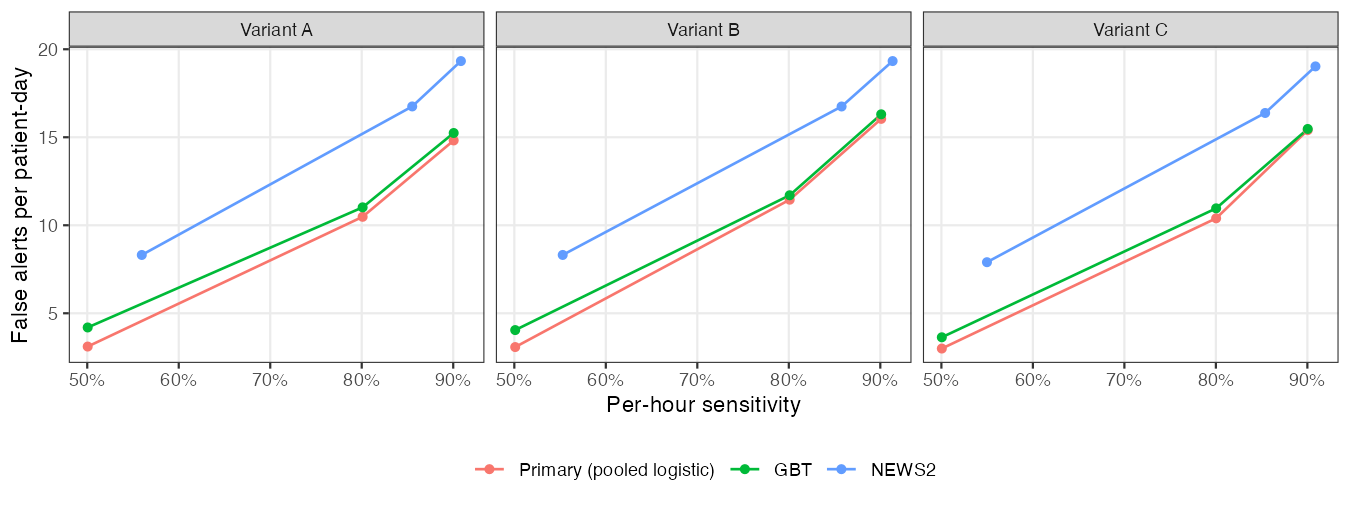
\includegraphics[width=\textwidth]{images/11_false_alarms_vs_sensitivity.png}
    \caption{False alerts per patient-day against per-hour sensitivity, at
    sensitivity targets of 50\%, 80\% and 90\%. The relationship is close to
    linear across the range.}
    \label{fig:fa_vs_sens}
\end{figure}

\subsection{Per-Patient (Event-Level) Detection \texorpdfstring{[C]}{[C]}}

Table~\ref{tab:patient_level} re-expresses the same operating points per
patient. Episode sensitivity within the actionable window counts a septic stay
as detected if any alert fired between six hours before onset and onset
itself. A false-alarm episode is a contiguous run of alert hours that does not
overlap the window from six hours before to three hours after onset, so a
five-hour alert run counts once rather than five times.

\begin{table}[H]
    \centering\small
    \adjustbox{max width=\textwidth}{%
    \begin{tabular}{llrrrrr}
        \toprule
        \textbf{Var} & \textbf{Model}
        & \textbf{Ep.\ sens (6\,h)} & \textbf{Ep.\ sens (any pre)}
        & \textbf{Patient PPV} & \textbf{\% stays alerted}
        & \textbf{FA ep./pt-day} \\
        \midrule
        A & Primary & \pcEpSensWindowPrimaryA & \pcEpSensPrePrimaryA & \pcPatientPpvPrimaryA & \pcPctStaysAlertedPrimaryA & \pcFaEpPerPtDayPrimaryA \\
        A & GBT     & \pcEpSensWindowGbtA & \pcEpSensPreGbtA & \pcPatientPpvGbtA & \pcPctStaysAlertedGbtA & \pcFaEpPerPtDayGbtA \\
        A & NEWS2   & \pcEpSensWindowNewsA & \pcEpSensPreNewsA & \pcPatientPpvNewsA & \pcPctStaysAlertedNewsA & \pcFaEpPerPtDayNewsA \\
        A & Cox     & \pcEpSensWindowCoxA & \pcEpSensPreCoxA & \pcPatientPpvCoxA & \pcPctStaysAlertedCoxA & \pcFaEpPerPtDayCoxA \\
        \midrule
        B & Primary & \pcEpSensWindowPrimaryB & \pcEpSensPrePrimaryB & \pcPatientPpvPrimaryB & \pcPctStaysAlertedPrimaryB & \pcFaEpPerPtDayPrimaryB \\
        B & GBT     & \pcEpSensWindowGbtB & \pcEpSensPreGbtB & \pcPatientPpvGbtB & \pcPctStaysAlertedGbtB & \pcFaEpPerPtDayGbtB \\
        B & NEWS2   & \pcEpSensWindowNewsB & \pcEpSensPreNewsB & \pcPatientPpvNewsB & \pcPctStaysAlertedNewsB & \pcFaEpPerPtDayNewsB \\
        B & Cox     & \pcEpSensWindowCoxB & \pcEpSensPreCoxB & \pcPatientPpvCoxB & \pcPctStaysAlertedCoxB & \pcFaEpPerPtDayCoxB \\
        \midrule
        C & Primary & \pcEpSensWindowPrimaryC & \pcEpSensPrePrimaryC & \pcPatientPpvPrimaryC & \pcPctStaysAlertedPrimaryC & \pcFaEpPerPtDayPrimaryC \\
        C & GBT     & \pcEpSensWindowGbtC & \pcEpSensPreGbtC & \pcPatientPpvGbtC & \pcPctStaysAlertedGbtC & \pcFaEpPerPtDayGbtC \\
        C & NEWS2   & \pcEpSensWindowNewsC & \pcEpSensPreNewsC & \pcPatientPpvNewsC & \pcPctStaysAlertedNewsC & \pcFaEpPerPtDayNewsC \\
        C & Cox     & \pcEpSensWindowCoxC & \pcEpSensPreCoxC & \pcPatientPpvCoxC & \pcPctStaysAlertedCoxC & \pcFaEpPerPtDayCoxC \\
        \bottomrule
    \end{tabular}}
    \caption{Per-patient detection at the 80\% per-hour sensitivity operating
    point, on \pcNTestStays{} test stays of which \pcNSepsisStaysA{} (A),
    \pcNSepsisStaysB{} (B) and \pcNSepsisStaysC{} (C) are septic. Ep.\ sens (6\,h): fraction of septic stays alerted
    within $[\text{onset}-6\,\text{h},\ \text{onset}]$. Ep.\ sens (any pre):
    alerted at any point before onset. FA ep./pt-day: false-alarm episodes,
    not alert-hours, per patient-day.}
    \label{tab:patient_level}
\end{table}

Under the primary label, \pcEpSensWindowPrimaryB{} of septic patients are
alerted inside the six-hour window and \pcEpSensPrePrimaryB{} at some point
before onset. Interpreted alone, patient-level detection obscures the
associated alert burden: to achieve it, the models alert on
\pcPctStaysAlertedCoxB--\pcPctStaysAlertedPrimaryA{} per cent of \emph{all}
stays. Patient-level PPV falls to \pcPatientPpvPrimaryB{} under Variant
B and \pcPatientPpvPrimaryC{} under Variant C, which are, to three decimal
places, the septic fractions of the cohort themselves
(\pcNSepsisStaysB/\pcNTestStays{} and
\pcNSepsisStaysC/\pcNTestStays). Because nearly every stay is alerted,
patient-level alerts provide little discrimination beyond the cohort
prevalence; under Variants A and C the primary model alerts on
\pcPctStaysAlertedPrimaryA{} per cent of the \pcNTestStays{} test stays.

\subsubsection{Per-Hour and Per-Patient, Side by Side}

\begin{table}[H]
    \centering\small
    \adjustbox{max width=\textwidth}{%
    \begin{tabular}{llrrrrrr}
        \toprule
        \textbf{Var} & \textbf{Model}
        & \textbf{Sens (hr)} & \textbf{Sens (pt)}
        & \textbf{PPV (hr)} & \textbf{PPV (pt)}
        & \textbf{FA hr/pt-day} & \textbf{FA ep./pt-day} \\
        \midrule
        A & Primary & \pcSensPrimaryA & \pcEpSensPrePrimaryA & \pcPpvPrimaryA & \pcPatientPpvPrimaryA & \pcFaPerPtDayPrimaryA & \pcFaEpPerPtDayPrimaryA \\
        A & GBT     & \pcSensGbtA & \pcEpSensPreGbtA & \pcPpvGbtA & \pcPatientPpvGbtA & \pcFaPerPtDayGbtA & \pcFaEpPerPtDayGbtA \\
        A & NEWS2   & \pcSensNewsA & \pcEpSensPreNewsA & \pcPpvNewsA & \pcPatientPpvNewsA & \pcFaPerPtDayNewsA & \pcFaEpPerPtDayNewsA \\
        \midrule
        B & Primary & \pcSensPrimaryB & \pcEpSensPrePrimaryB & \pcPpvPrimaryB & \pcPatientPpvPrimaryB & \pcFaPerPtDayPrimaryB & \pcFaEpPerPtDayPrimaryB \\
        B & GBT     & \pcSensGbtB & \pcEpSensPreGbtB & \pcPpvGbtB & \pcPatientPpvGbtB & \pcFaPerPtDayGbtB & \pcFaEpPerPtDayGbtB \\
        B & NEWS2   & \pcSensNewsB & \pcEpSensPreNewsB & \pcPpvNewsB & \pcPatientPpvNewsB & \pcFaPerPtDayNewsB & \pcFaEpPerPtDayNewsB \\
        \midrule
        C & Primary & \pcSensPrimaryC & \pcEpSensPrePrimaryC & \pcPpvPrimaryC & \pcPatientPpvPrimaryC & \pcFaPerPtDayPrimaryC & \pcFaEpPerPtDayPrimaryC \\
        C & GBT     & \pcSensGbtC & \pcEpSensPreGbtC & \pcPpvGbtC & \pcPatientPpvGbtC & \pcFaPerPtDayGbtC & \pcFaEpPerPtDayGbtC \\
        C & NEWS2   & \pcSensNewsC & \pcEpSensPreNewsC & \pcPpvNewsC & \pcPatientPpvNewsC & \pcFaPerPtDayNewsC & \pcFaEpPerPtDayNewsC \\
        \bottomrule
    \end{tabular}}
    \caption{The same operating point viewed per person-hour and per patient.
    Across these rows the two views differ by more than twentyfold in PPV and
    by roughly tenfold in alarm count.}
    \label{tab:hour_vs_patient}
\end{table}

Per-hour PPV of \pcPpvPrimaryB{} and per-patient PPV of
\pcPatientPpvPrimaryB{} describe one model at one threshold on one test set.
The choice of denominator changes the reported PPV by a factor of twenty-six,
more than the spread attributed to label definition (H1) or model class (H6),
so it is an analyst decision that requires pre-specification.

\subsection{Lead Time to Onset \texorpdfstring{[C]}{[C]}}

Lead time is the interval between the first alert issued at or before onset
and the onset hour, over septic stays that were alerted at all.

\begin{table}[H]
    \centering\small
    \begin{tabular}{llrrrr}
        \toprule
        \textbf{Var} & \textbf{Model} & \textbf{Median (h)} & \textbf{IQR (h)}
        & \textbf{$\geq 3$\,h} & \textbf{$\geq 6$\,h} \\
        \midrule
        A & Primary & \pcLeadMedianPrimaryA & \pcLeadQXXVPrimaryA--\pcLeadQLXXVPrimaryA & \pcFracLeadGeThreePrimaryA & \pcFracLeadGeSixPrimaryA \\
        A & GBT     & \pcLeadMedianGbtA & \pcLeadQXXVGbtA--\pcLeadQLXXVGbtA & \pcFracLeadGeThreeGbtA & \pcFracLeadGeSixGbtA \\
        A & NEWS2   & \pcLeadMedianNewsA & \pcLeadQXXVNewsA--\pcLeadQLXXVNewsA & \pcFracLeadGeThreeNewsA & \pcFracLeadGeSixNewsA \\
        A & Cox     & \pcLeadMedianCoxA & \pcLeadQXXVCoxA--\pcLeadQLXXVCoxA & \pcFracLeadGeThreeCoxA & \pcFracLeadGeSixCoxA \\
        \midrule
        B & Primary & \pcLeadMedianPrimaryB & \pcLeadQXXVPrimaryB--\pcLeadQLXXVPrimaryB & \pcFracLeadGeThreePrimaryB & \pcFracLeadGeSixPrimaryB \\
        B & GBT     & \pcLeadMedianGbtB & \pcLeadQXXVGbtB--\pcLeadQLXXVGbtB & \pcFracLeadGeThreeGbtB & \pcFracLeadGeSixGbtB \\
        B & NEWS2   & \pcLeadMedianNewsB & \pcLeadQXXVNewsB--\pcLeadQLXXVNewsB & \pcFracLeadGeThreeNewsB & \pcFracLeadGeSixNewsB \\
        B & Cox     & \pcLeadMedianCoxB & \pcLeadQXXVCoxB--\pcLeadQLXXVCoxB & \pcFracLeadGeThreeCoxB & \pcFracLeadGeSixCoxB \\
        \midrule
        C & Primary & \pcLeadMedianPrimaryC & \pcLeadQXXVPrimaryC--\pcLeadQLXXVPrimaryC & \pcFracLeadGeThreePrimaryC & \pcFracLeadGeSixPrimaryC \\
        C & GBT     & \pcLeadMedianGbtC & \pcLeadQXXVGbtC--\pcLeadQLXXVGbtC & \pcFracLeadGeThreeGbtC & \pcFracLeadGeSixGbtC \\
        C & NEWS2   & \pcLeadMedianNewsC & \pcLeadQXXVNewsC--\pcLeadQLXXVNewsC & \pcFracLeadGeThreeNewsC & \pcFracLeadGeSixNewsC \\
        C & Cox     & \pcLeadMedianCoxC & \pcLeadQXXVCoxC--\pcLeadQLXXVCoxC & \pcFracLeadGeThreeCoxC & \pcFracLeadGeSixCoxC \\
        \bottomrule
    \end{tabular}
    \caption{Lead time at the 80\% sensitivity operating point. The
    $\geq 3$\,h and $\geq 6$\,h columns are fractions of \emph{all} septic
    stays, not only detected ones.}
    \label{tab:lead_time}
\end{table}

\begin{figure}[H]
    \centering
    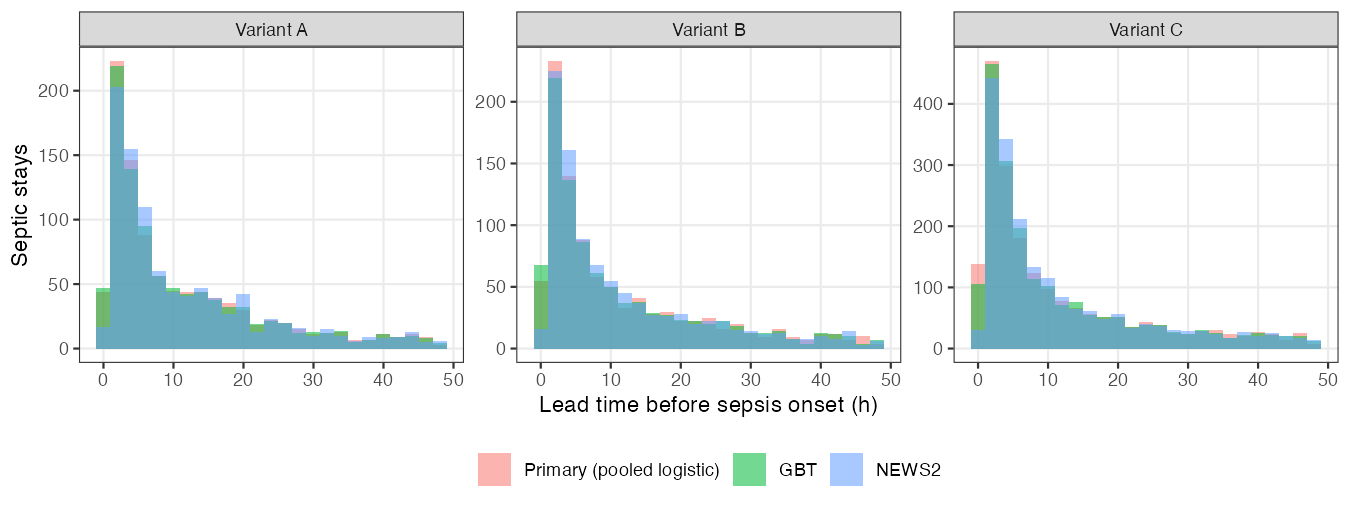
\includegraphics[width=\textwidth]{images/11_lead_time_distribution.png}
    \caption{Distribution of lead time before onset at the 80\% sensitivity
    operating point, truncated at 48 h. The mode lies in the first four hours,
    with a long right tail. Because almost every stay is alerted at this
    operating point, the distribution is not evidence of advance warning.}
    \label{fig:lead_time}
\end{figure}

Median lead time is \pcLeadMedianPrimaryC--\pcLeadMedianPrimaryB{} hours for
the primary model, with \pcFracLeadGeSixPrimaryB{} of septic stays alerted at
least six hours ahead under the primary label, but nearly every stay is
alerted at this operating point. The long lead-time tail
(Figure~\ref{fig:lead_time}) therefore includes alerts unrelated to the
subsequent onset, and these estimates are not comparable with the 4--12 hour
horizons in the literature \cite{henry2015trewscore, moor2023review}. They
should not be interpreted as evidence of actionable advance warning without
controlling alert burden.
